\providecommand{\main}{..}
\documentclass[\main/main.tex]{subfiles}
\begin{document}
\chapter{Technologies}
\section{Distributed computing}
\subsection{MapReduce}
\subsection{Spark}

\section{Transformers}
Transformers \allowbreak\cite{vaswani2017attention} are an architecture based only on attention mechanism, dispensing with recurrence and convolutions. Transformers are used to draw global dependencies between input and output.
\subsection{Architecture}
\begin{figure}[h]
    \centering
    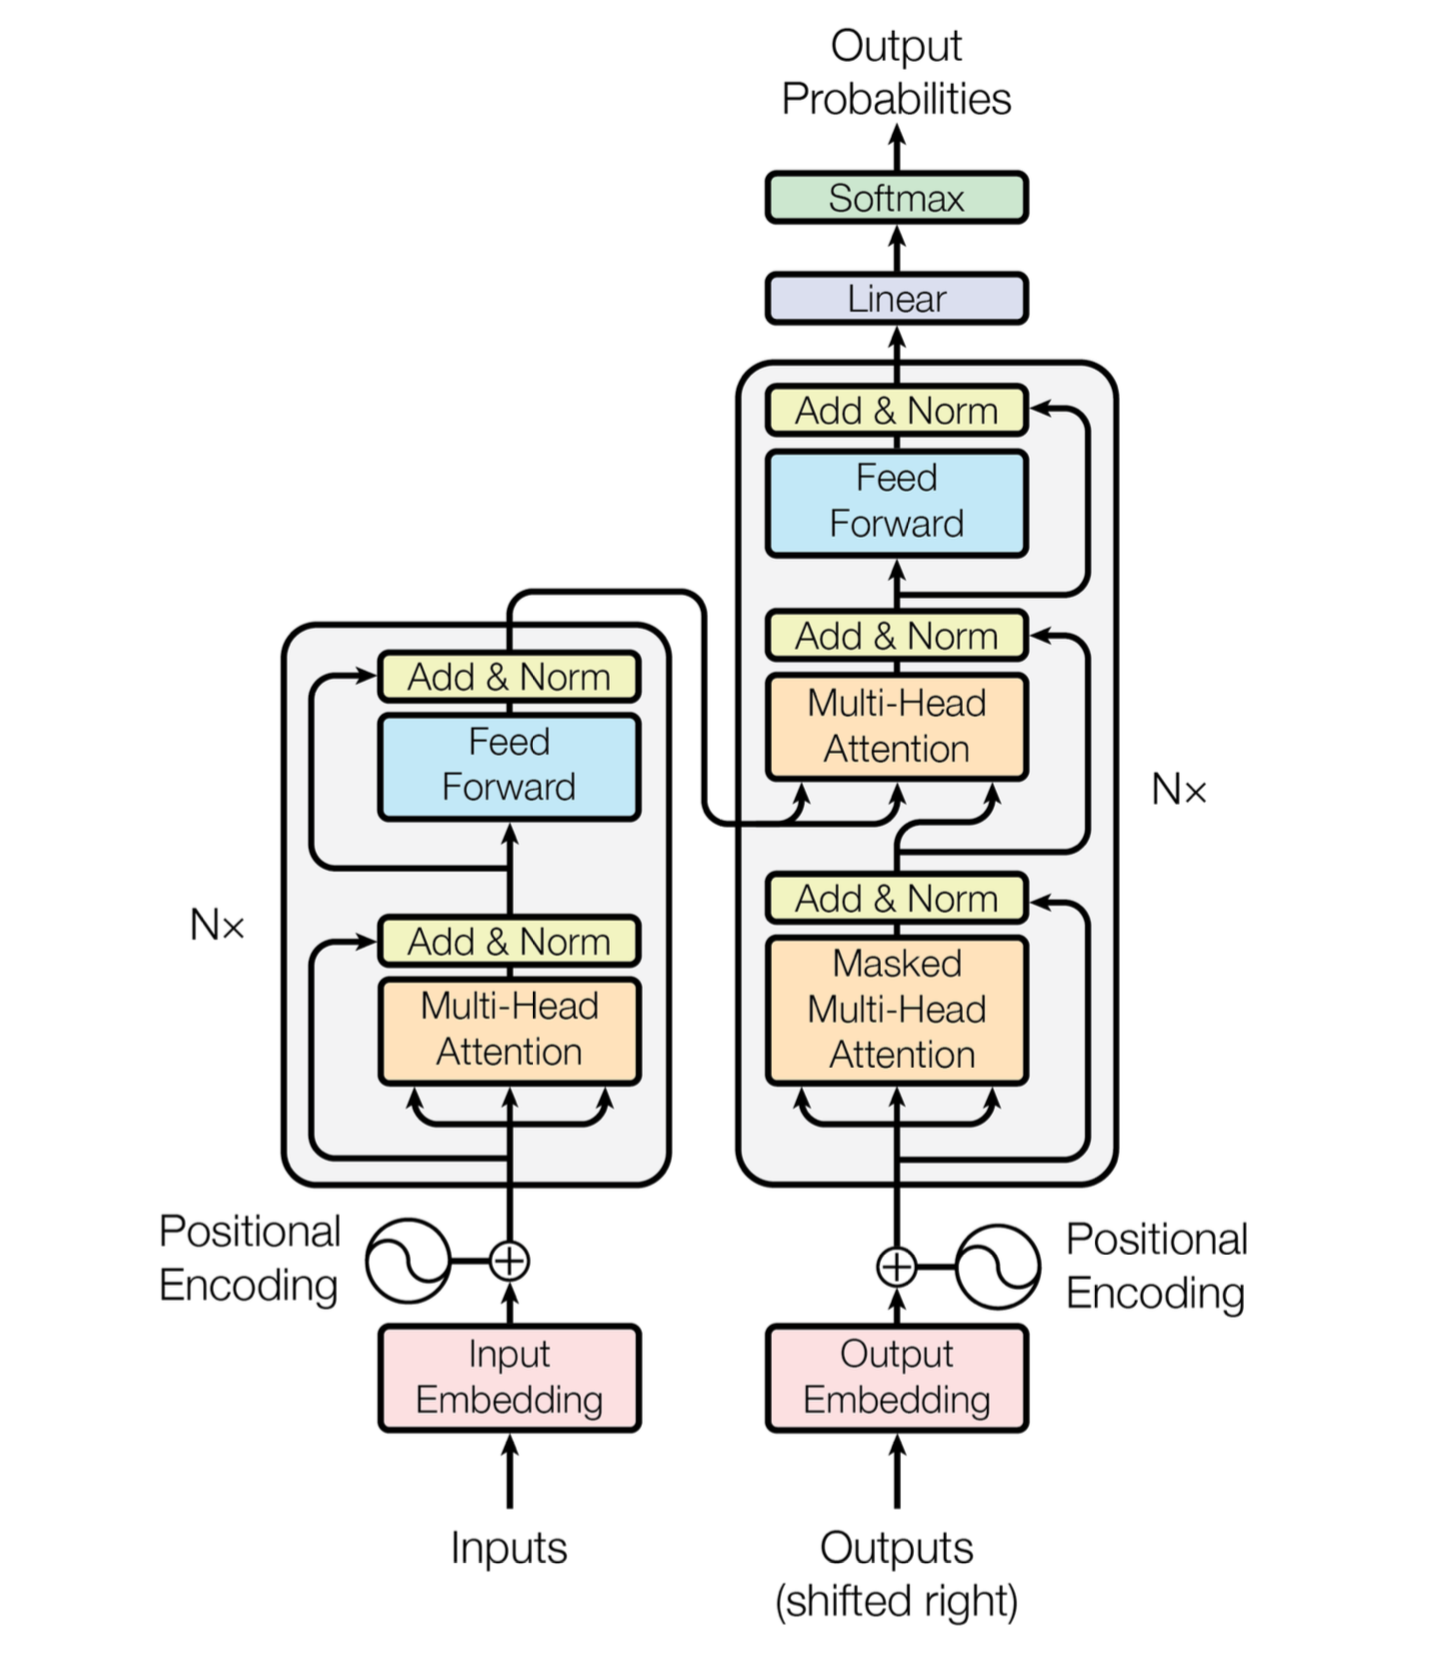
\includegraphics[scale=0.35]{images/transformer/transformer_model_architecture.png}
    \caption{Transformer architecture}
    \label{fig:transformer_architecture}
\end{figure}

Transformers, like most competitive neural sequence transduction, have an encoder-decoder structure with the encoder mapping to an input sequence of symbols $(x_1, \dots, x_n)$ to a continuous representation $z = (z_1, \dots, z_n)$. Given $z$, the decoder generates an output sequence $(y_1, \dots, y_m)$ of symbols one element at a time. In the left and right halves of Figure \ref{fig:transformer_architecture} is shown the fully-connected layers of both encoders and decoders.
\subsection{Encoder}
The encoder is composed of a stack of $N=6$ identical layers, each one has two sub-layers:
\begin{itemize}
    \item a multi-head self-attention mechanism
    \item a position-wise fully connected feed-forward network
\end{itemize}
\todo[inline]{finish encoder}
\subsection{Decoder}
The decoder is composed of a stack of $N=6$ identical layers. The decoder inserts a third sub-layer to the two encoder sub-layer. This sub-layer performs multi-head attention over the output of the encoder stack.
\todo[inline]{finish decoder}
\subsection{Attention}
An attention function consists in mapping a query and a set of key-value pairs to an output, where the query, keys, values and output are all vectors. The output is computed as a weighted sum of the values, with weights computed by a compatibility function of the query with the corresponding key.
\subsubsection{Scaled dot-product attention} 
\begin{figure}[h!]
    \centering
    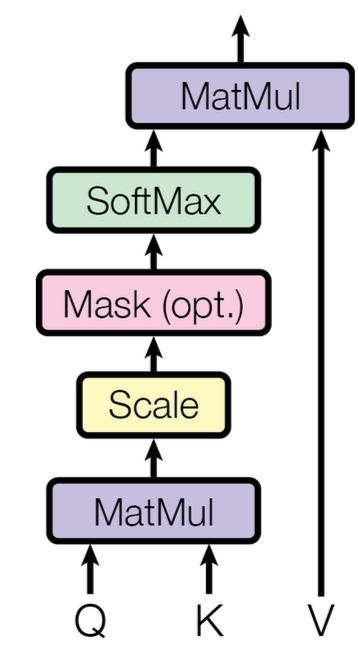
\includegraphics[scale=0.35]{images/transformer/scaled_dot_product_attention.png}
    \caption{Scaled dot-product attention}
    \label{fig:scaled_dot-product_attention}
\end{figure}
The input consists of queries and keys of dimension $d_k$, and values of dimension $d_v$.
To obtain the weights on the values, the dot product of the query with all keys is performed, dividing each by $\sqrt{d_k}$ and applying a softmax function.
The queries, values and keys sets are packed together into Q (queries), K (keys) and V (values) sets. 
The attention function is computed using Q, K and V matrices, producing an output matrix in this way:
\begin{center}
    $Attention(Q, K, V) = softmax(\frac{QK^T}{\sqrt{d_k}})V$
\end{center}
Scaled dot-product attention is both faster and more space efficient of two commonly used attention functions: additive attention and dot-product (multiplicative) attention. These performances reachable because of the highly optimized implementation of matrix multiplication code.
\subsubsection{Multi-head attention}
\begin{figure}[h]
    \centering
    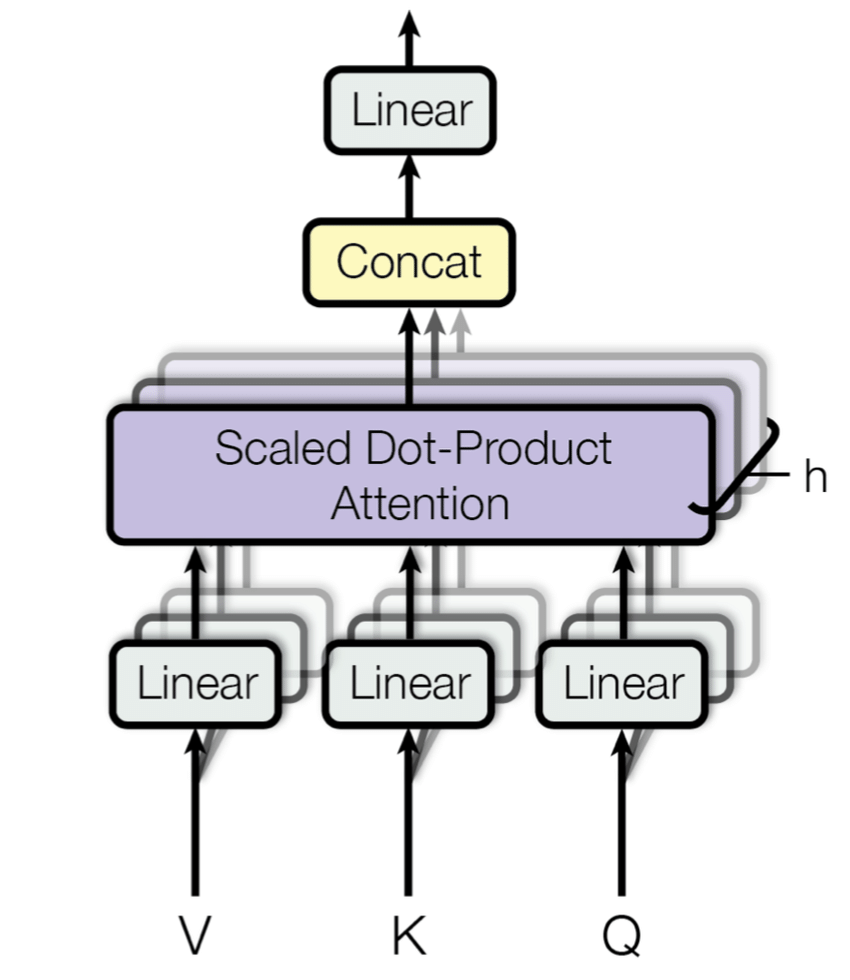
\includegraphics[scale=0.25]{images/transformer/multi-headed_attention.jpeg}
    \caption{Multi-head attention}
    \label{fig:multi-head_attention}
\end{figure}
As visible in Figure \ref{fig:multi-head_attention}, queries, values and keys are linearly projected $h$ times, with different learned linear projections to $d_k$, $d_q$ and $d_v$ dimensions respectively. The attention function is performed in parallel on each projection, yielding $d_v$-dimensional output values. These are concatenated and once again projected, resulting in the final values. \\
Multi-head attention allows the model to jointly attend to information form different representation subspaces at different position. 
\begin{center}
    $MultiHead(Q, V, K) = Concat(head_1, \dots, head_h)W^O$\\
    where $head_i = Attention(QW^Q_i, KW^K_i, VW^V_i)$
\end{center}
Where the projections are parameter matrices $W^Q_i\in\R^{d_{model \times d_k}}, W^K_i\in\R^{d_{model \times d_k}}, W^V_i\in\R^{d_{model \times d_k}}$ and $ W^O_i\in\R^{d_{model \times d_k}}$.

\subsection{Position-wise Feed-Forward Networks}
Every layer in both encoders and decoders contain a fully connected feed-forward neural network, which is applied to each position separately and identically.
It consists of two linear transformations with a ReLU activation in between.
\begin{center}
    $FFN(x) = max(0, xW_1 + b_1)W_2 + b_2$
\end{center}
The linear transformations remain the same across different positions, using different parameters on each layer. 
\todo[inline]{finish this part while writing other models}

\subsection{Transformer technology in language field}
Transformer technology and its bidirectional training have been used in the language modeling field. BERT \cite{devlin2018bert} is the first application of training bidirectionality in language representation field.
\subsubsection{BERT}
\subsubsection{MPNET}
\subsubsection{XLM}





\end{document}